\chapter{Design and implementation}
\label{chap:design-and-implementation}

\defaultInstructions

\begin{length}
There are no strict length requirements for this chapter.  However, it is important that the writing is clear and concise.  Avoid repeating yourself.  Make sure to clearly signpost evidence for claims.  It should be possible for a reader to understand this chapter without consulting other sources.  It is expected that a typical project needs 3--6 pages, but this can vary considerably from project to project.
\end{length}

\begin{expectations}
In this chapter, the team should discuss the key design and implementation decisions made during the project, and how these are reflected in the end product.  Design refers to the way the software system is organised into smaller components and the way in which they are related.  We are \emph{not} looking for a discussion of a series of screenshots of your application.

Normally, all teams should present the overall architecture of the software.  The remainder of the chapter will depend on the type of system that is built.  To decide what to cover, consider the following to aspects of the project:
\begin{itemize}
\item What design and implementation decisions did you make to improve software quality?
\item What design and implementation decisions did you make to achieve challenging functional and non-functional specifications
\end{itemize}
Depending on your answers to these questions, you may cover the design an implementation specific components, interfaces, the overall class structure, the database design, algorithms, business processes, etc.

A good report considers alternative options for key decisions and includes sound justifications for the decisions made.  If applicable, you may reflect on changes made during the project.  Ideally, key decisions are rooted in Software Engineering theory.
\end{expectations}

\section{Design and Implementation}

This section discusses how our software is designed and implemented, focusing on meeting both functional requirements (such as creating and managing habits) and non-functional requirements (such as security, maintainability, and reliability). We outline the three-tier architecture and explain our rationale for each design choice, demonstrating how the client, server, and database work together.

\subsection{Overall Architecture}

Our system uses a three-tier structure: \begin{itemize} \item \textbf{Client (React Native and Expo)}:
Displays user interfaces for activities like logging in, managing habits, and viewing calendars or statistics. We use Expo Router to organise screens.
\item \textbf{Server (Node.js and Express)}:
Provides REST endpoints (for example, /signup, /addHabit, /export/:email) to handle authentication, validate user data, and manage business logic.
\item \textbf{Database (MySQL via mysql2/promise)}:
Stores user credentials, habit definitions, scheduling information, and user progress records. \end{itemize}

\begin{figure}[H]
    \centering
    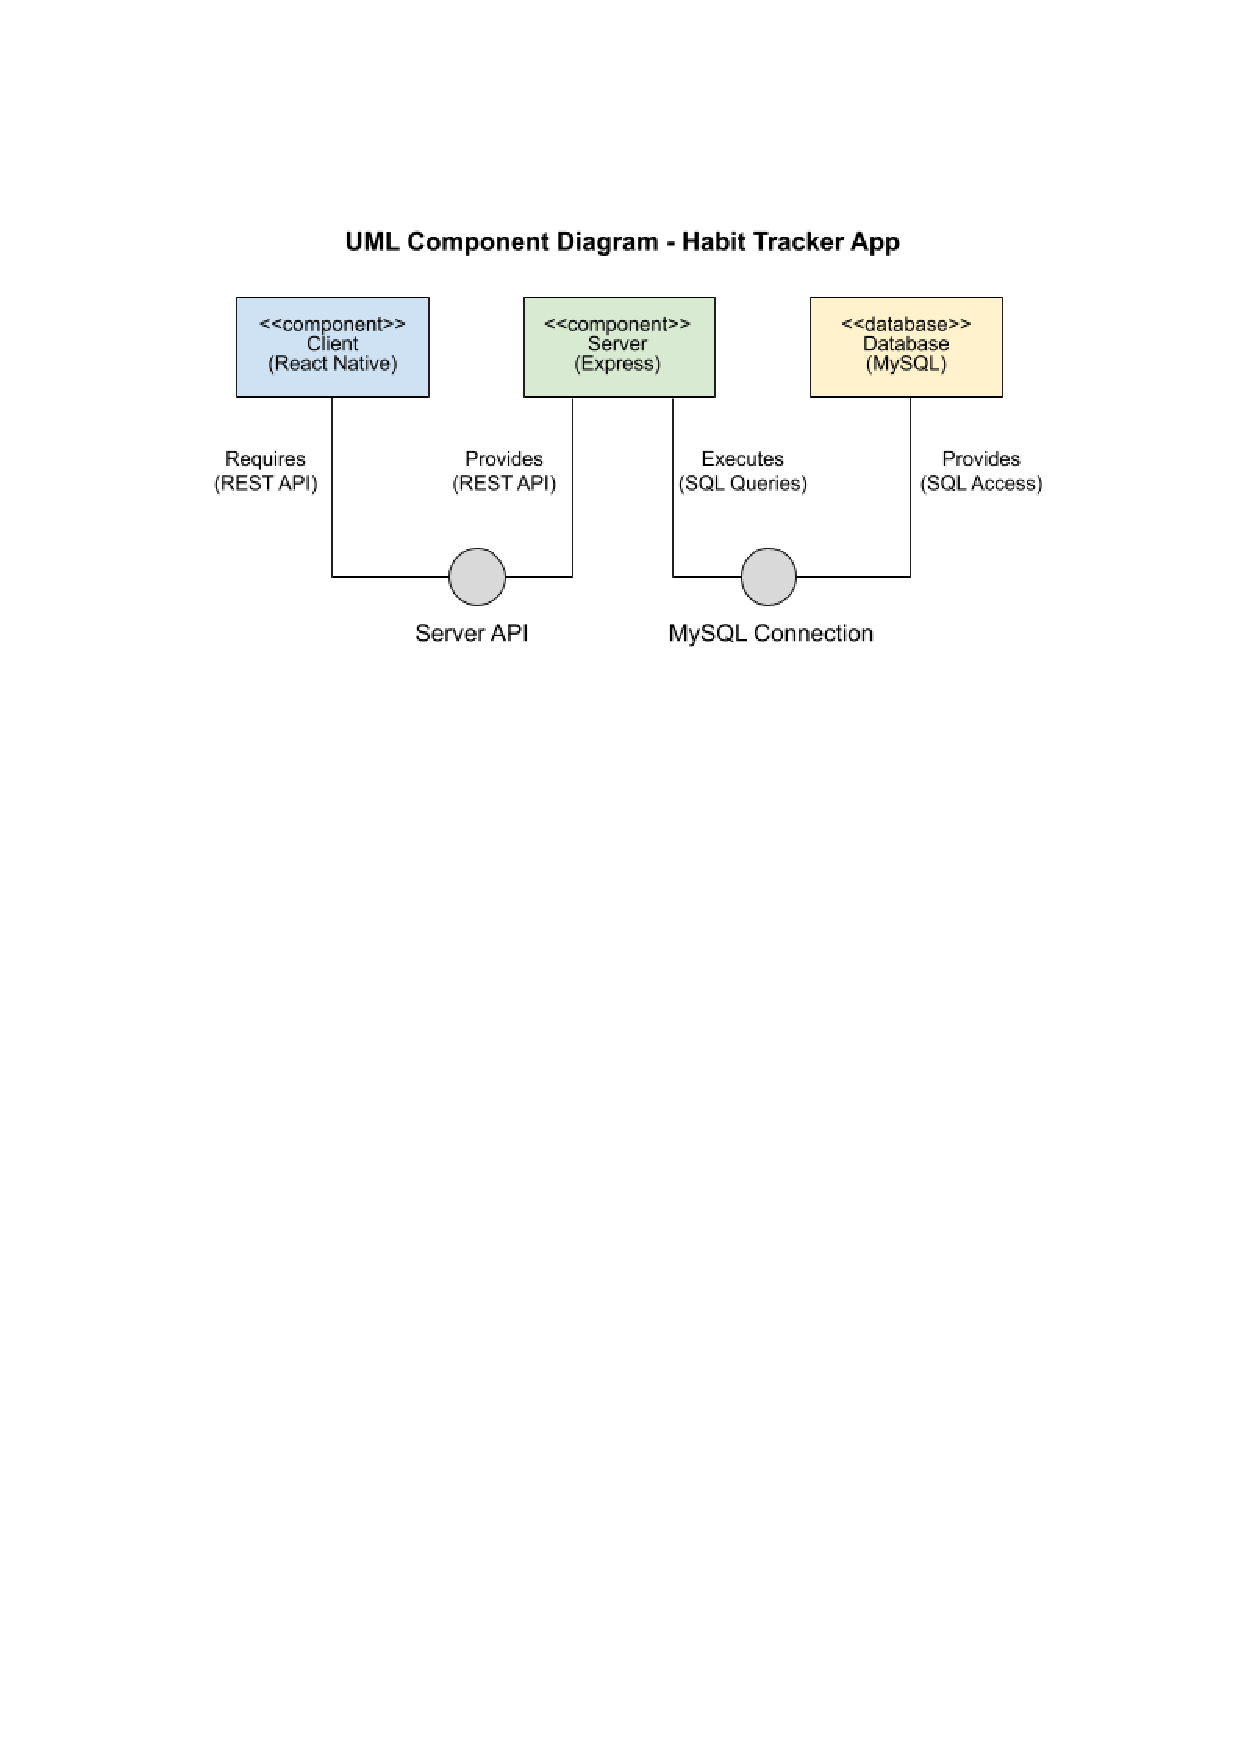
\includegraphics[width=0.7\textwidth]{resources/component.pdf}
    \caption{UML Component Diagram of our Habit-Tracker Application}
    \label{fig:component_diagram}
\end{figure}

Figure 5.1 illustrates these layers. By separating the UI (client), the application logic (server), and storage (database), each layer remains independently maintainable and secure.

\subsection{Key Design Decisions}

\subsubsection{Cross-Platform Client Using Expo:}

\paragraph{Choice and Reasoning} \begin{itemize} \item We wanted a single codebase (TypeScript) for iOS, Android, and web accessibility, which is why we chose React Native and Expo.
\item Expo simplifies building and testing on multiple platforms, preventing the need for a complicated setup. This allowed us to start developing features much sooner, rather than spending time on configuration.  \end{itemize}

\paragraph{Implementation Details} \begin{itemize} \item {File Structure}:
\begin{itemize} \item {src/app/(auth)/}: Handles login and signup screens.
\item{src/app/(protected)/tabs/}: Contains the main habits, calendar, stats, and settings screens.
\item{src/components/}: Contains reusable UI elements such as habit modals, calendars, graphs, themed text, and shared styles for consistent design.
\item {src/lib/client.ts}: Centralises HTTP request logic to avoid repeating fetch calls across components. \end{itemize} 
This modular structure improves code organisation, makes features easier to maintain, and encourages reuse of components across the app.
\item {Styling and Theming}:
\begin{itemize} 
\item The app uses shared colours and styles so that all screens look consistent.
\item Common layouts, buttons, and inputs are defined in reusable style files to avoid repeating code.
\item Some components automatically change their appearance based on the selected theme (light or dark), making the app easier to use and nicer to look at. \end{itemize} \end{itemize}


\subsubsection{Server with Node.js and Express:}

\paragraph{Choice and Reasoning}
\begin{itemize}
\item Node.js and Express were chosen because they are widely used, beginner-friendly, and well-supported by online documentation and learning resources.
\item Express enables a simple and flexible REST API structure, making it easy to define endpoints that connect to application features like signing up, adding habits, or exporting data.
\end{itemize}

\paragraph{Implementation Details}
\begin{itemize}
\item Express is used to define REST endpoints such as \texttt{/signup}, \texttt{/addHabit}, and \texttt{/export/:email}, which the client interacts with to manage user accounts and habits.
\item Middleware like \texttt{cors} and \texttt{dotenv} help with handling requests, loading environment settings, and allowing the mobile app to connect to the server.
\item Authentication uses JSON Web Tokens (JWT) to protect routes and make sure only logged-in users can access certain features.
\end{itemize}

\subsubsection{MySQL Database:}

\paragraph{Choice and Reasoning}
\begin{itemize}
  \item A relational database structure is ideal for managing related entities such as users, habits, and habit completion logs. MySQL allows us to enforce clear relationships and constraints through primary and foreign keys.
  
  For example, in the habit\_progress table, a foreign key constraint on (user\_email, habitName) references the habits table. This ensures that progress entries cannot exist without a matching habit, and enables automatic cleanup of related records when a habit is deleted, maintaining data integrity.

  \item We use the \texttt{mysql2/promise} library to write our own SQL commands directly (such as \texttt{CREATE TABLE} and \texttt{SELECT}) and run them using modern \texttt{async/await} syntax. This gives us full control over database operations, and keeps the code clean, readable, and easier to debug.
\end{itemize}

\paragraph{Schema Outline}\mbox{}\\
Below is an overview of some of the main tables that make up our database schema.
\begin{itemize}

  \item {users}: Stores user account information. The \texttt{email} field acts as the primary key and is used to identify users. Each user also has a hashed password and a username.

  \item {habits}: Stores details about each habit a user creates. Each habit is uniquely identified by a combination of \texttt{user\_email} and \texttt{habitName}, which together form a composite primary key. Other fields include habit type (build or quit), goal settings, and scheduling options (e.g., interval or weekly).

  \item {habit\_progress}: Logs daily progress for each habit. The composite primary key (\texttt{user\_email}, \texttt{habitName}, \texttt{progressDate}) ensures that only one record exists per user, habit, and date. This table tracks goal progress, completion status, and streak count. A foreign key links back to the \texttt{habits} table, ensuring referential integrity.

\item {habit\_days}: Supports weekly habit scheduling. Each record maps a habit to a day of the week (e.g., Monday, Wednesday). This allows habits to repeat on specific days, and also uses a foreign key to maintain referential integrity with the \texttt{habits} table.

\end{itemize}

\begin{figure}[H]
    \centering
    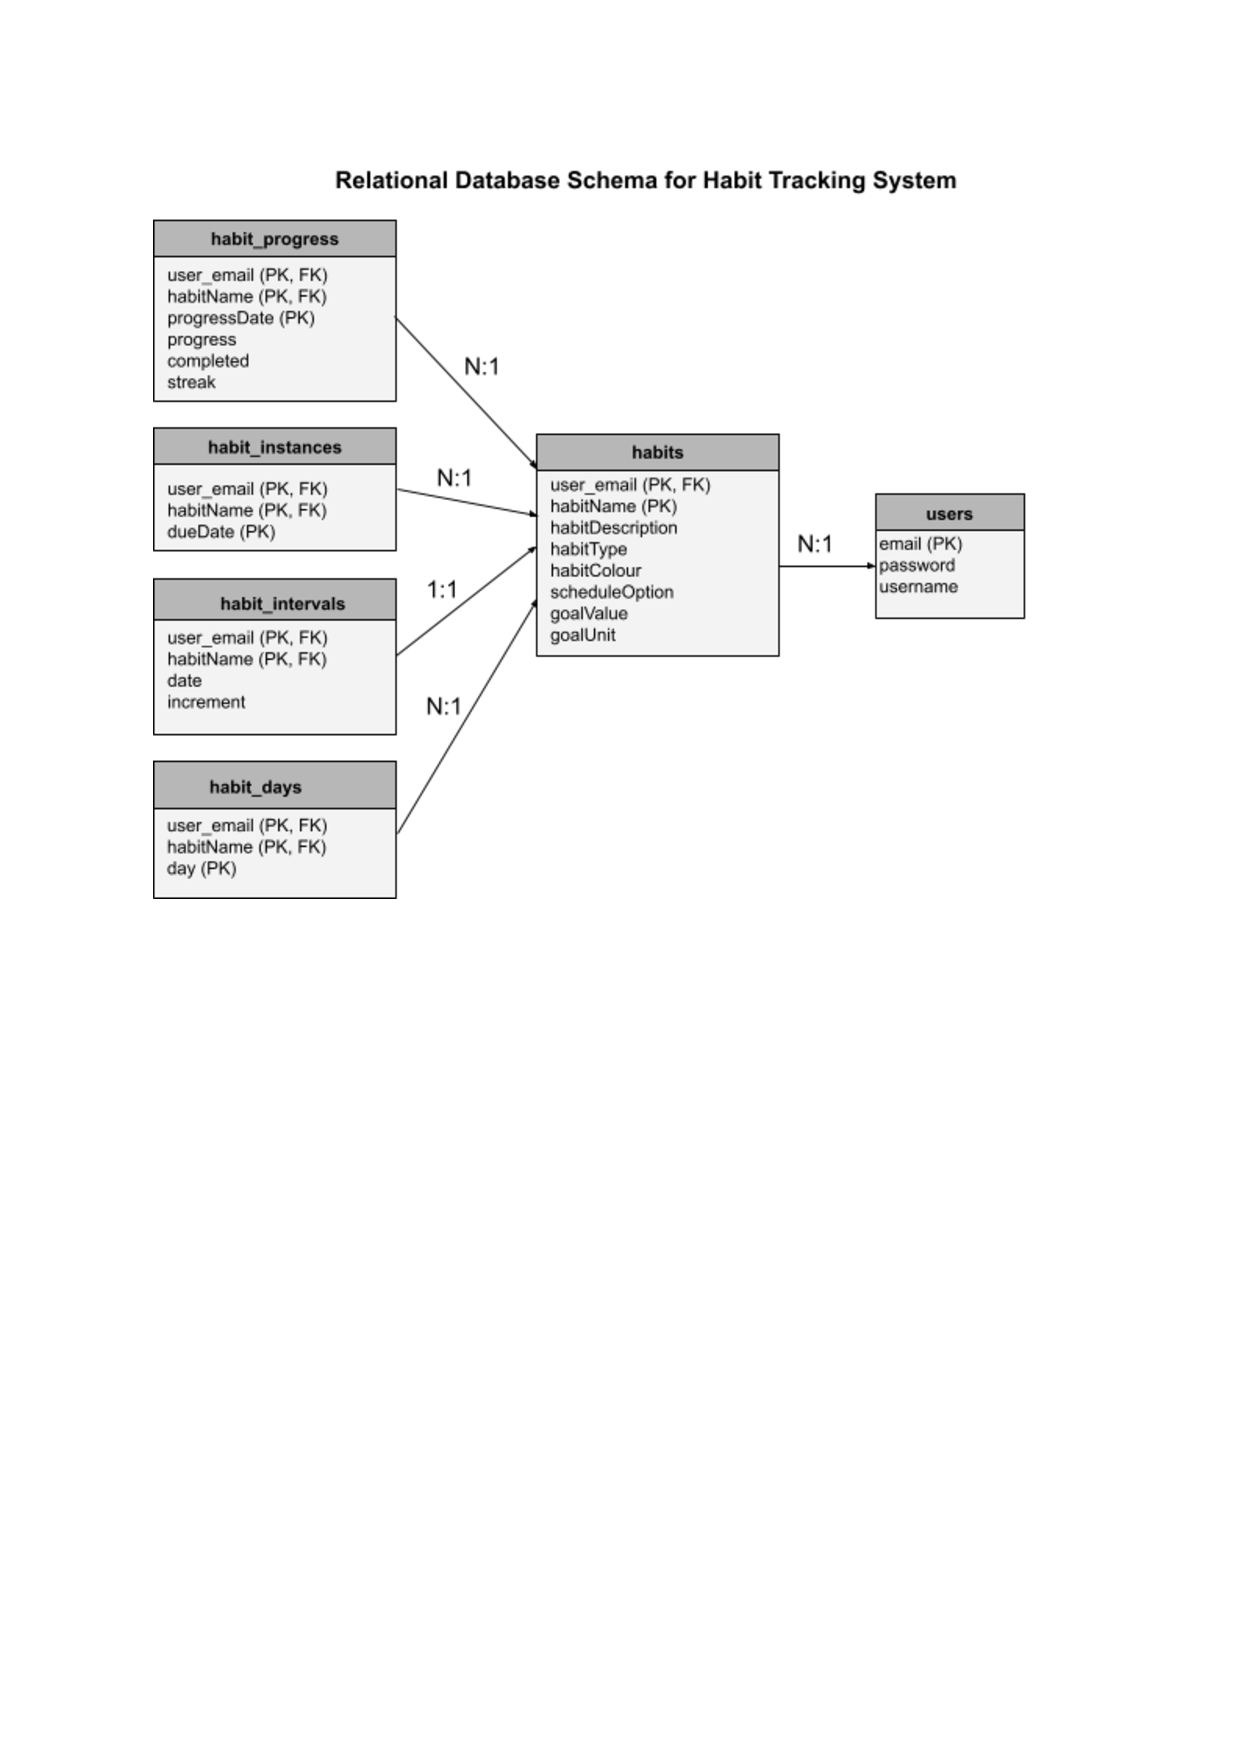
\includegraphics[width=0.9\textwidth]{resources/database_schema.pdf}
    \caption{Relational Database Schema of our Habit Tracking System}
    \label{fig:database_schema}
\end{figure}

Figure 5.2 shows the tables in the habit-tracking database and their relationships. Arrows represent foreign keys, and cardinality ratios (e.g., 1:1, N:1) indicate how records in one table relate to others, supporting data integrity and structure.

\section{Meeting Requirements}

This section summarises some examples of how our system design and implementation meet the project's key functional and non-functional requirements (as specified in Chapter 3 of this report). We focus on how our architecture, database structure, and code design support these goals (instead of just listing all the features).

\subsection{Functional Requirements}

\begin{itemize}
  \item \textbf{Habit Creation and Management:} Users can create, customise, and update habits with flexible scheduling (interval-based or weekly), goals, and visual settings. These features are implemented through reusable client components and backed by structured database tables (\texttt{habits}, \texttt{habit\_progress}, \texttt{habit\_days}).

  \item \textbf{Progress Tracking and Visualisation:} The system calculates and displays daily progress, streaks, and completion trends via calendar views and graphs. These visual features reflect real-time data stored and retrieved from the backend.

  \item \textbf{Data Export:} A dedicated API endpoint (\texttt{/export/:email}) allows users to download their habit history in JSON format, so users can view and save a copy of their own data.
\end{itemize}

\subsection{Non-Functional Requirements}


\begin{itemize}
  \item \textbf{Security:} All user passwords are hashed client-side before being sent to the server. Routes requiring authentication use JSON Web Tokens (JWT), and all data operations go through validated REST endpoints.

  \item \textbf{Maintainability:} The codebase is modular, with clear separation between client, server, and database logic. Client-side fetch logic is centralised, and components follow single-responsibility principles for easier reuse and testing.

  \item \textbf{Performance and Scalability:} We use SQL with \texttt{mysql2/promise} to make database queries fast and efficient. Composite keys and foreign key links help keep the data consistent and quick to access.

  \item \textbf{Data Integrity:} Relationships between tables are enforced through composite foreign keys. For example, \texttt{habit\_progress} entries reference existing habits, and \texttt{ON DELETE CASCADE} ensures cleanup when habits are removed.
\end{itemize}


\section{Alternative Approaches}

Throughout development, we considered several alternative technologies and approaches:

\begin{itemize}
  \item {Using an ORM}: ORMs can make database tasks easier, but we chose to write SQL ourselves using \texttt{mysql2/promise} to have more control over scheduling logic and table relationships like composite keys and foreign keys.

  \item {Native iOS/Android Development}: We considered building separate native apps for each platform, but chose React Native with Expo to keep one shared codebase. This made development easier and faster, while also allowing the app to run smoothly on iOS, Android, and the web.
\end{itemize}


\section{Conclusion}

Our design and implementation emphasise a three-tier architecture that separates the user interface, server-side logic, and database.
The result is a cross-platform habit-tracking application that cleanly meets project needs for scheduling, progress tracking, data visualisation, and security measures. The system is also designed to be easily extended in the future, with potential additions like advanced analytics, social features, or smarter notifications.
